%%%%%
\begin{figure}[!ht]
\centering
  \hfill\subfloat[ii=24]{
  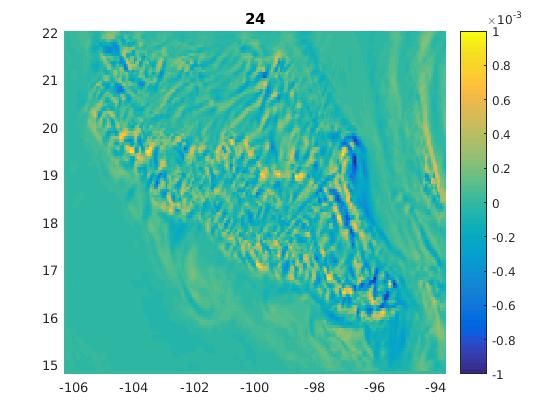
\includegraphics[width=0.35\textwidth]{t3rot1}
  }\hfill
  \subfloat[ii=29]{%\label{fig:}
  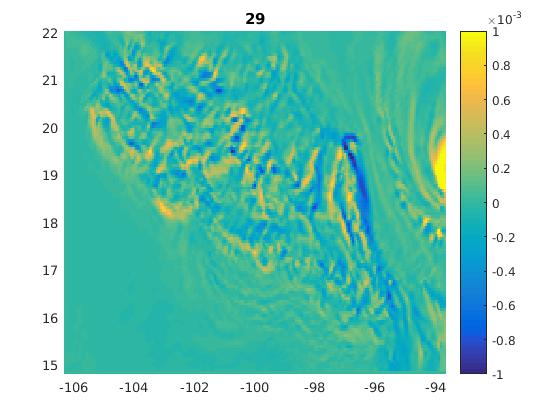
\includegraphics[width=0.35\textwidth]{t3rot2}
  }\hfill

  \hfill\subfloat[ii=34]{
  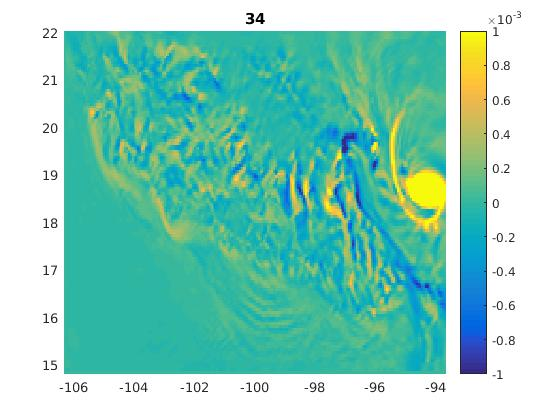
\includegraphics[width=0.35\textwidth]{t3rot3}
  }\hfill
  \subfloat[ii=39]{%\label{fig:}
  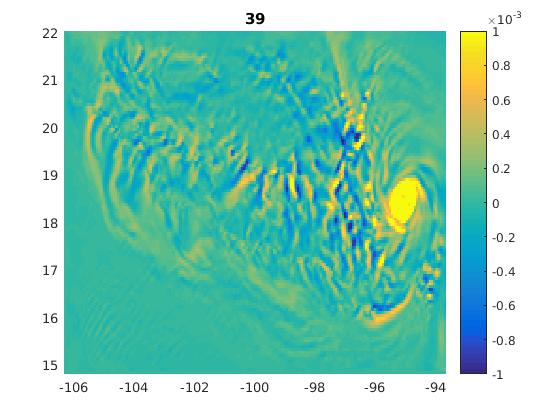
\includegraphics[width=0.35\textwidth]{t3rot4}
  }\hfill
  \caption{Rotacional en 4 tiempos distintos, se calcula sobre una superfice (nivel 8) y esto implica que s\'olo resulte una componente que es perpendicular a la superficie, el rotacional sigue la regla de la mano derecha y es proporcional a la velocidad angular.}%
\label{fig:tres}
\end{figure}
%%%%%